\section{}
Zbudowano licznik modulo 16. Ręcznie wyzwalając wejście licznika za pomocą impulsatora znajdującego się na płytce UC-1, zaobserwowano kolejne stany licznika ukazane poprzez diody LED.
Zaobserwowano również podział częstotliwości sygnału prostokątnego podanego generatorem przez \(2^n\), gdzie \(n\) jest kolejnym bitem wyjściowym licznika.

\begin{figure}[H]
    \centering
    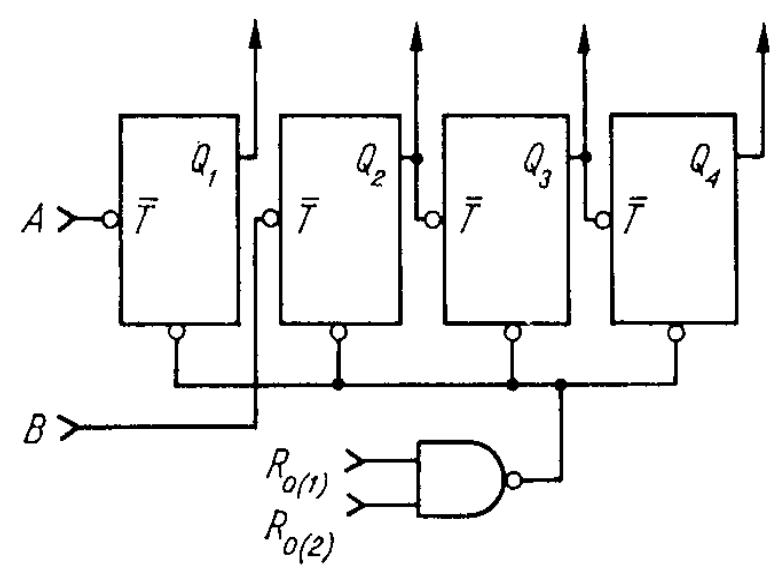
\includegraphics[width=7.5cm]{include/5/1.png}
    \caption{Schemat logiczny układu UCY7493.}
\end{figure}

Do budowy licznika wykorzystano układ UCY7493, aby połączyć wszystkie 4 zawarte w nim przerzutniki w szereg tworzący licznik, połączono ze sobą wyprowadzenia \(Q_1\) i \(B\). Wyprowadzenie \(A\) stało się wejściem licznika, na wejścia resetujące \(R_0\) i \(R_1\) podano stan wysoki. Licznik cyklicznie przechodzi przez wszystkie możliwe stany, których jest \(2^4=16\).